\documentclass[11pt]{article}%other possible arguments are book, report, thesis etc..
%\usepackage{times}
\usepackage[top=1in, bottom=1in, left=0.5in, right=0.5in]{geometry}
\usepackage{graphicx}
\title{Physics Behind Simulation: A CS296 Report by Group 28}
\author{Venkata Dinesh (120050051)\\
\texttt {dineshkota3@cse.iitb.ac.in}\and
Nitish Chandra (120050071)\\
\texttt{nitish@cse.iitb.ac.in}\and
Kota Mahindar (120050073)\\
\texttt{mahindar@cse.iitb.ac.in}
}
%\maketitle
\begin{document}
\date{\today}
\maketitle
\section{Introduction}
%The main purpose of this report is to analyse the expected behaviour of objects in a physical world
%The verbal description of this simulation\newline\begin{listing}
\begin{itemize}
\item To understand every object used in this simulation. They are represented in this report with the help of picture and figures.
\item To know what is going to happen when one object interacts with other.
\item To understand the physics involved in interaction of objects with the help of principles and formulae involved in it.
\item To know about the constraints and restrictions of moving objects in the simulation.
\end{itemize}
\section{Physics Behind Simulation}
%\subsection*{Square Pendulum}
%The main idea behind the present analysis is that any force through the center of mass of the body doesn't produce any tourque around center of mass.
\subsection{Falling Rod}
Initially, the rod is in between the bob of the pendulum and the dominos. Due to gravity, the rod falls onto the ground. Since the \emph{coefficient of restitution} $$e=0$$ it sticks to the ground without getting reflected.
%\noindent 
For simplicity, let us assume that the mass of rod is $M$, length of the rod is $l$, mass of the ball is $m$ and the speed of the ball is $v$. 

Let us calculate the impulse imparted about Center of Mass(CM) produced on the rod due to its collision with the ball. Let the final velocity of the ball just after collision is $v_a$.
Therefore the momentum exchanged is \begin{equation}\Delta p=mv-mv_a\end{equation} therefore impulse imparted is\cite{kleppner} \begin{equation} L = \Delta p\cdot \left(l\over 2\right)\end{equation}

Using conservation of momentum in x direction, we get \begin{equation}(\Delta p)_{x of CM}+\Delta p=0\end{equation}
where, $(\Delta p)_{x of CM}$ is the change in momentum of Center of Mass of the rod.
\vskip 1in 
\centerline{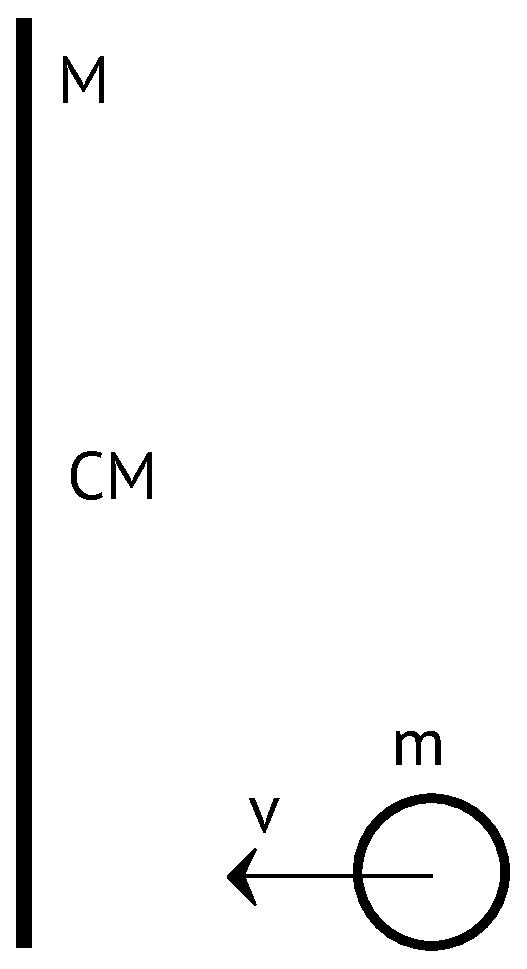
\includegraphics[scale=0.3, trim=0in 0in 0in 2in]{topplingrod}}

Due to this impulse, the rod starts to rotate and due to gravity $g$, it also starts to fall.
\vskip 0.5in
\centerline{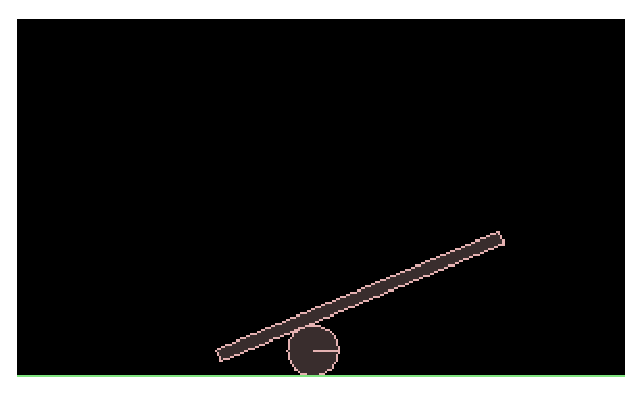
\includegraphics[scale=0.7]{toppledexec}}
\vskip 0.3in
\subsection{Balls in the Box}
Initially, a ball is on the top of another ball. Let the mass of each ball be $m$ and the mass of the box be $M$.Both the balls and the open box doesn't have any velocity in the horizontal direction. So, total initial momentum in the horizontal direction is zero.\begin{equation}\sum_{i=1}^3p_i=0\end{equation} 
Throughout the motion of the system, there is no horizontal force. Therefore by definition of \it force\rm\cite{hcverma},\begin{equation}F_{ext}= {d\sum p_i\over\displaystyle dt}\end{equation}

Since, \begin{equation}F_{ext}=0\end{equation}
\centerline{$\displaystyle \sum_{i=1}^3p_i$ is constant throughout the motion of the system.}

\vskip 0.2in
\centerline{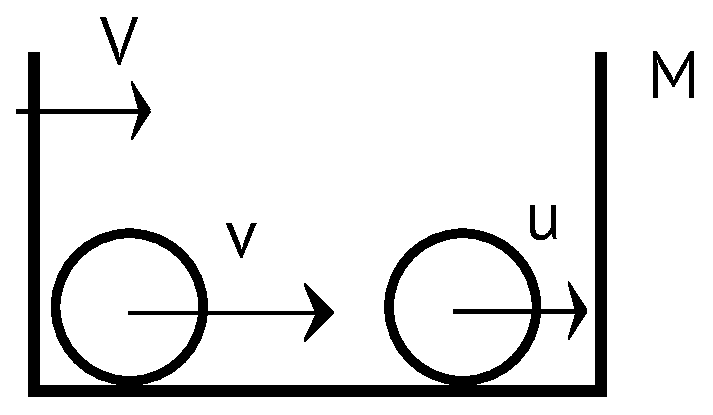
\includegraphics[scale=0.4]{dubdubdub}}

Let the velocities of the balls, at a given instance $t$ be $u$ and $v$ respectively and the velocity of the box be $V$ as shown. Therefore, the equation governing the motion of the system at a given time is\begin{equation}mv+mu+MV\end{equation} is constant throughout the motion.
\vskip 0.5in
\centerline{
\includegraphics[scale=1.1]{dubdubexec}}
\vskip 0.3in
\subsection{Rotating square pendulum}
A square pendulum is attatched to an anchor and the pendulum is free to rotate around its own Center of Mass. Firstly, pendulum starts to rotate around itself because of the impulse given to it by the ball hitting the square.

Let the mass of the ball be $m$ and the mass of square bob be $M$. If the ball hits with a speed of $v$ and after the collision, it has a speed of $v_a$, change in momentum \begin{equation}\Delta p = mv_a-mv\end{equation}
Therefore, angular impulse $L$ imparted to the square pendulum is \begin{equation}L=\Delta p\cdot d\end{equation} where $d$ is the vertical distance between Center of Mass of square and the point of impact. 
The angular velocity imparted depends on \emph{moment of inertia} $I$ of the bob.\begin{equation}I\omega=L\end{equation}
%\vskip 0.1in
\centerline{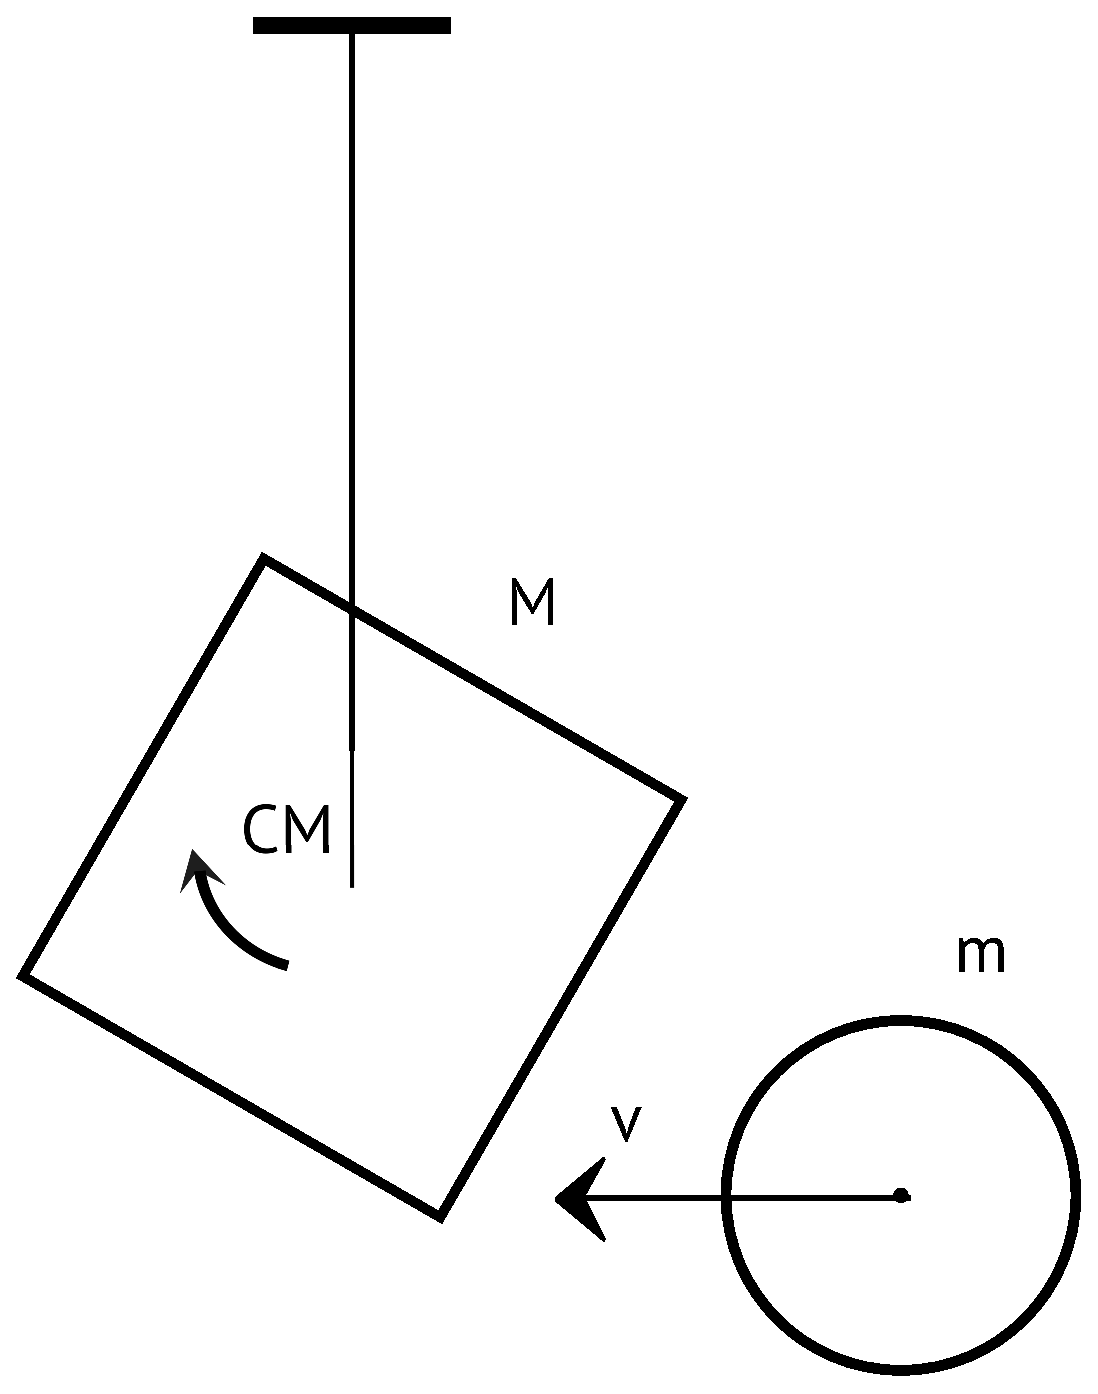
\includegraphics[scale=0.2]{sqpendulumnotexec}}
Conservation of momentum indicates that the momentum imparted to the bob is $\Delta p$. Due to the constraint of fixed distance between anchor and Center of Mass, the bob starts to revolve around the anchor point.

Once the motion starts, the revolution around the anchor point is driven by the force of gravity. The gravitational force on the bob acts through the Center of Mass of the bob. Therefore, the Torque imparted about Center of Mass $\Gamma$ is zero.\begin{equation}\Gamma_{ext}=0\end{equation}

Therefore, by the definition of \emph{angular momentum L}, \begin{equation}\Gamma_{ext}={dL\over dt}\end{equation}
the angular momentum of the square remains constant forever.\cite{resnick}
\vskip 0.5in
\centerline{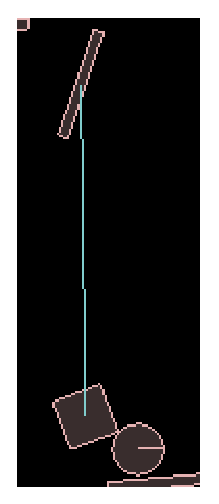
\includegraphics[scale=0.8]{sqpendulumexe}}
\vskip 0.3in
\section{Conclusions}
All the three systems added to \tt dominos.cpp \rm are explained with the behaviour is expected in their respective physical situations.
%\vskip 2in
%\section{References}
%THis is basically%\cite{lamport94} nothing more than nothing
%\begin{thebibliography}{9}
%\bibitem{LaTeXsource}
%\tt http://en.wikipedia.org/wiki/TeX
%\bibitem{TeXsource}
%The TeXbook by Donald Knuth
%\bibitem{lamport9a4}
%Leslie Lamport, \emph{\LaTeX: something here}.
%The most wanted publishers.

%\end{thebibliography}
\bibliographystyle{plain}
\bibliography{cs296_report_28}
\end{document}
